%!TEX TS-program=xelatex
\documentclass[xetex]{beamer}

\usefonttheme{professionalfonts}
\usepackage[UTF8]{ctex}
\usepackage{hyperref}
\usepackage{unicode-math}
\usepackage{amsmath, amssymb}
\usepackage{graphicx, wrapfig}
\usepackage{nopageno}

\DeclareMathOperator{\argmax}{argmax}

\usetheme[block=fill, subsectionpage=progressbar]{metropolis}

\setmathfont{XITS Math}

%这是标题页
\title{重积分}
\subtitle{重积分的变量代换}
\author{数学分析MOOC小组 }
\date{}
%这是标题页

\begin{document}

\frame{\maketitle}

\begin{frame}
    \frametitle{回顾:定积分的变量代换}
    若$f(x)$在$[a,b]$连续,变量代换$x=\varphi(t)$在$\alpha\leq t \leq\beta$可微,$\varphi(\alpha)=a,\varphi(\beta)=b$,则
    $$\int_a^bf(x)\,\mathrm{d}x=\int_{\alpha}^{\beta}f(\varphi(t))\varphi^\prime(t)\,\mathrm{d}t$$
\end{frame}

\begin{frame}
    \frametitle{一种导数表示}
    有变量代换
    $$\begin{cases}
        x=\varphi(u,v)\\
        y=\psi(u,v)
    \end{cases}$$
    则有,
    $$J(u,v)=\dfrac{\partial(x,y)}{\partial(u,v)}=
        \begin{vmatrix}
             \dfrac{\partial\varphi}{\partial u} & \dfrac{\partial \varphi}{\partial v} \\
             \dfrac{\partial\psi}{\partial u} & \dfrac{\partial \psi}{\partial v}
         \end{vmatrix}
         $$
\end{frame}

\begin{frame}
    \frametitle{重积分变量代换定理}
    设变换$T:$
    $$\begin{cases}
        x=\varphi(u,v)\\
        y=\psi(u,v)
    \end{cases}$$
    把$Ouv$平面上由逐段光滑的闭曲线围成的区域$\Delta$一一映射为$Oxy$平面的区域$D$,且$\varphi,\psi$在$\Delta$有二阶连续偏导数,
    \begin{center}
    $J(u,v)=\dfrac{\partial(x,y)}{\partial(u,v)}\neq0$ \quad 当$(u,v)\in\Delta$,
    \end{center}
    而$f(x,y)$是定义在$D$上的连续函数,则
    $$\iint\limits_Df(x,y)\,\mathrm{d}x\mathrm{d}y=\iint\limits_{\Delta}f(\varphi(u,v),\psi(u,v))|J(u,v)|\,\mathrm{d}u\mathrm{d}v$$
\end{frame}

\begin{frame}
    \frametitle{极坐标代换}
    做变换
    $$\begin{cases}
        x=r\cos{\theta}\\
        y=r\sin{\theta}
    \end{cases}$$
    变换的函数行列式为
    $$\dfrac{\partial(x,y)}{\partial(r,\theta)}=
    \begin{vmatrix}
        \cos{\theta} & -r\sin{\theta} \\
        \sin{\theta} & r\cos{\theta}
    \end{vmatrix}
    =r$$
    计算公式
    $$\iint\limits_Df(x,y)\,\mathrm{d}x\mathrm{d}y=\iint\limits_{\Delta}f(r\cos{\theta},r\sin{\theta})r\,\mathrm{d}r\mathrm{d}\theta$$
\end{frame}

\begin{frame}
    \frametitle{极坐标代换例题}
    $\displaystyle \iint\limits_D(x^2+y^2)\,\mathrm{d}x\mathrm{d}y$,$D$由双纽线$(x^2+y^2)^2=a^2(x^2-y^2)(x\geq 0)$围成。\pause

    做变换
    $$\begin{cases}
        x=r\cos{\theta}\\
        y=r\sin{\theta}
    \end{cases}$$
    原函数变为
    $$r = a \sqrt{\cos{2 \theta}} $$
    $$- \frac{\pi}{4} < \theta < \frac{\pi}{4}, \quad 0 \leq r \leq a \sqrt{\cos{2 \theta}} $$
\end{frame}
    
\begin{frame}
    \frametitle{极坐标代换例题}
    \begin{figure}[ht]
        \centering %图片居中放置
        % 在这里使用 \includegraphics 插入图片,改变width就可以改变图片的大小。
       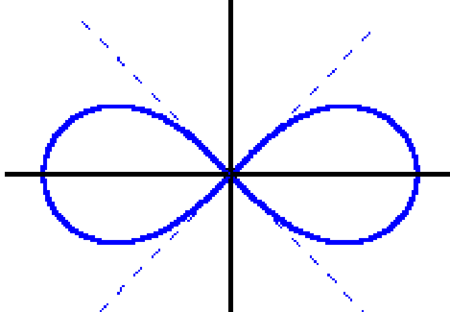
\includegraphics[width=0.5\textwidth]{img/c.jpg}
    \end{figure}
    \pause
    解:
    \begin{align*} 
        \iint \limits_D (x^2 + y^2) \,\mathrm{d}x\mathrm{d}y &= \int _{ - \frac{4}{\pi} } ^{ \frac{4}{\pi} } \,\mathrm{d} \theta \int _0 ^{a \sqrt{ \cos{2 \theta} } } r^3 \,\mathrm{d}r = \frac{a^2} {4} \int  _{ - \frac{4}{\pi} } ^{ \frac{4}{\pi} } \cos ^2 {2 \theta} \,\mathrm{d} \theta \\
        &= \frac {a^2} {8} \int _{ - \frac{4}{\pi} } ^{ \frac{4}{\pi} } (1+ \cos{4 \theta}) \,\mathrm{d} \theta = \frac{\pi} {16} a^2
    \end{align*}
\end{frame}

\begin{frame}
    \frametitle{极坐标代换例题}
    求椭球体的体积$V$,椭球体为
    $$\dfrac{x^2}{a^2}+\dfrac{y^2}{b^2}+\dfrac{z^2}{c^2}\leq1$$
    \pause
    由对称性知,
    $$V=2\iint\limits_Dc\sqrt{1-\frac{x^2}{a^2}-\frac{y^2}{b^2}}\,\mathrm{d}x\mathrm{d}y$$
    \begin{center}
    其中$D=\left\{(x,y) \left| \dfrac{x^2}{a^2}+\dfrac{y^2}{b^2}\leq1 \right.\right\}.$
    \end{center}
\end{frame}    

\begin{frame}
    \frametitle{极坐标代换例题}
    做广义极坐标变换
    $$x=ar\cos{\theta}, y=br\sin{\theta}$$
    则$D$对应于$0\leq r \leq1, 0\leq\theta\leq2\pi.$而
    $$J(r,\theta)=\dfrac{\partial (x,y)}{\partial (r,\theta)}=
        \begin{vmatrix}
             a\cos{\theta} & -ar\sin{\theta} \\
             b\sin{\theta} & br\cos{\theta}
         \end{vmatrix}
         =abr$$
\end{frame}  

\begin{frame}
    \frametitle{极坐标代换例题}
    因此
    \begin{align*}
    V &= 2\int _0 ^{2 \pi} \,\mathrm{d} \theta \int _0^1 c \sqrt{1 - r^2} abr\,\mathrm{d}r \\
      &=4 \pi abc \int _0 ^1 \sqrt{1 - r^2} r\,\mathrm{d}r \\
      &= \left. 4 \pi abc \frac{1}{2} \cdot \frac{2}{3} (1 - r^2) ^{\frac{3}{2}} \right| _1 ^0 \\
      &= \frac{4}{3} \pi abc
     \end{align*}
\end{frame} 

\begin{frame}
    \frametitle{三重积分的变量代换}
    做变换
    $$\begin{cases}
         x=x(u,v,w) \\
         y=y(u,v,w) \\
           z=z(u,v,w)
    \end{cases} $$   
    则
    \begin{align*}
    &\iiint\limits_V f(x,y,z) \,\mathrm{d}x\mathrm{d}y\mathrm{d}z \\
    = &\iiint\limits_\Omega f(x(u,v,w), y(u,v,w), z(u,v,w)) \left| \dfrac{\partial (x,y,z)}{\partial (u,v,w)} \right|\,\mathrm{d}u\mathrm{d}v\mathrm{d}w
    \end{align*}
\end{frame} 

\begin{frame}
    \frametitle{柱坐标代换}
    变换
    $$\begin{cases}
        x=r \cos{\theta} & 0 \leq r < + \infty \\
        y=r \sin{\theta} & 0 \leq  \theta < 2 \pi \\
        z=z & - \infty < z < + \infty
    \end{cases}$$
    这时
    $$J(r , \theta , z) = \dfrac{\partial (x,y,z)}{\partial (r, \theta ,z)} = 
    \begin{vmatrix}
        \cos{\theta} & -r\sin{\theta} & 0 \\
        \sin{\theta} & r\cos{\theta} & 0 \\
        0  & 0 & 1
    \end{vmatrix} = r$$
    PS:$z$不变,$x,y$变为对应的极坐标。
\end{frame} 

\begin{frame}
    \frametitle{柱坐标代换}
    因此变量代换公式为
    $$\iiint \limits_V f(x,y,z) \,\mathrm{d}x\mathrm{d}y\mathrm{d}z =  \iiint \limits_{\Omega} f(r \cos{\theta} , r \sin{\theta} , z) r\,\mathrm{d}r\mathrm{d} \theta \mathrm{d}z$$
\end{frame} 

\begin{frame}
    \frametitle{球坐标代换}
    做变换
    $$\begin{cases}
        x = r \cos{\theta} \sin{\varphi} & 0 \leq r < + \infty \\
        y = r \sin{\theta} \sin{\varphi} & 0 \leq \theta < 2 \pi \\
        z = r \cos{\varphi} & 0 \leq \varphi \leq \pi \\
    \end{cases}$$
    PS: $\theta$代表经度,$\varphi$代表维度,$r$代表与地心的距离。\\
    \begin{figure}[ht]
        \centering %图片居中放置
        % 在这里使用 \includegraphics 插入图片,改变width就可以改变图片的大小。
       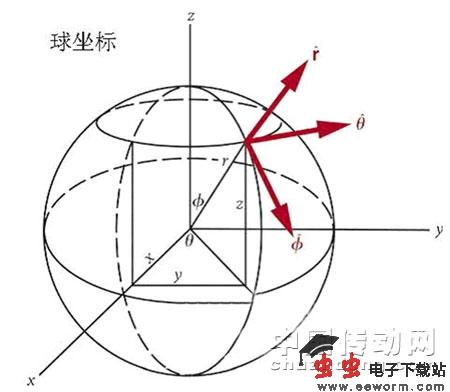
\includegraphics[width=0.4\textwidth]{img/g.jpg}
    \end{figure}
\end{frame} 

\begin{frame}
    \frametitle{球坐标代换}
    这时
    \begin{align*}
         J(r , \theta , \varphi) &= \dfrac {\partial (x,y,z)} {\partial (r, \theta , \varphi)} \\
         &=
         \begin{vmatrix}
             \cos{\theta} \sin{\varphi} & -r \sin{\theta} \sin{\varphi} & r \cos{\theta} \cos{\varphi} \\
             \sin{\theta} \sin{\varphi} & r \cos{\theta} \sin{\varphi} & r \sin{\theta} \cos{\varphi} \\
             \cos{\varphi} & 0 & -r \sin{\varphi} 
         \end{vmatrix} = - r^2 \sin{\varphi}
    \end{align*} 
     因此变量代换公式为
    \begin{align*}
        &\iiint \limits_V f(x,y,z) \,\mathrm{d}x\mathrm{d}y\mathrm{d}z \\
        =  &\iiint \limits_{\Omega} f(r \cos{\theta} \sin{\varphi} , r \sin{\theta} \sin{\varphi} , r \cos{\varphi}) r^2        \sin{\varphi} \,\mathrm{d}r\mathrm{d} \theta \mathrm{d} \varphi
    \end{align*}
\end{frame} 

\begin{frame}
    \frametitle{三重坐标代换例题}
    作适当的变量代换,求下列三重积分:

    $$\iiint\limits_Vx^2y^2z\,\mathrm{d}x\mathrm{d}y\mathrm{d}z$$
    $V$是由$$\displaystyle z=\frac{x^2+y^2}{a},z=\frac{x^2+y^2}{b},xy=c,xy=d,y=\alpha x,y=\beta x$$围成的立体,其中$0<a<b,0<c<d,0<\alpha<\beta$。
\end{frame} 

\begin{frame}
    \frametitle{三重坐标代换例题}

    解:作变换$\displaystyle u=\frac{x^2+y^2}{z},v=xy,w=\frac{w}{x}$,则变换把$V$变为
    $$\Delta: a\leq u\leq b,c\leq v\leq d, \alpha\leq w\leq\beta$$
    逆变换为$\displaystyle x=\sqrt{\frac{v}{w}},y=\sqrt{wv},z=\sqrt{\frac{v(1+w^2)}{uw}}$。

    $$\therefore \frac{\partial(u,v,w)}{\partial(x,y,z)}=\begin{vmatrix}
        \frac{2x}{z} & \frac{2y}{z} & -\frac{x^2+y^2}{z^2} \\
        y & x & 0 \\
        -\frac{y}{x^2} & \frac{1}{x} & 0
    \end{vmatrix}=-\frac{x^2+y^2}{z^2}\cdot\frac{2y}{x}=-2v(1+w^2)$$
    $$\therefore J(u,v,w)=-\frac{1}{2v(1+w^2)}$$

\end{frame}

\begin{frame}
    \frametitle{三重坐标代换例题}

    \begin{align*}
        \iiint\limits_Vx^2y^2z\,\mathrm{d}x\mathrm{d}y\mathrm{d}z 
        &= \iiint\limits_\Delta\frac{v^3(1+w^2)}{uw}\cdot\frac{1}{2v(1+w^2)}\,\mathrm{d}u\mathrm{d}v\mathrm{d}w \\
        &= \iiint\limits_\Delta\frac{v^2}{2uw}\,\mathrm{d}u\mathrm{d}v\mathrm{d}w \\
        &= \frac{1}{2}\int_a^b\frac{\mathrm{d}u}{u}\cdot\int_c^dv^2\,\mathrm{d}v\cdot\int_\alpha^\beta\frac{\mathrm{d}w}{w} \\
        &= \frac{d^3-c^3}{6}\ln\frac{b}{a}\ln\frac{\beta}{\alpha}
    \end{align*}

\end{frame}

\begin{frame}
    \section{谢谢观看!}
\end{frame} 

\end{document}